\section{Tutorial A3}

\begin{problem}
    If $a$, $b$, $c$ are sides of a triangle, show that \[\frac{a}{b+c-a} + \frac{b}{a+c-b} + \frac{c}{a + b - c} \geq 3.\]
\end{problem}
\begin{proof}
    Let \[x = \frac{a + b - c}2, \quad y = \frac{b + c - a}2, \quad z = \frac{c + a - b}2.\] By the triangle inequality, we have $x, y, z > 0$. Hence, by AM-GM, \[2\sqrt{xy} \leq x + y, \quad 2\sqrt{yz} \leq y + z, \quad 2\sqrt{zx} \leq z + x,\] so \[8xyz \leq (x+y)(y+z)(z+x).\] Replacing $x, y, z$ with their corresponding definitions in $a, b, c$, we get \[\frac{(x+y)(y+z)(z+x)}{8xyz} = \frac{abc}{\bp{b + c - a} \bp{a + c - b} \bp{a + b - c}} \geq 1.\] Thus, by AM-GM, \[\frac{a}{b+c-a} + \frac{b}{a+c-b} + \frac{c}{a + b - c} \geq \frac{3abc}{\bp{b + c - a} \bp{a + c - b} \bp{a + b - c}} \geq 3\] as desired.
\end{proof}

\begin{problem}
    \begin{enumerate}
        \item For some positive integer $n$, let $x_1 \leq x_2 \leq \dots \leq x_n$ and $y_1 \leq y_2 \leq \dots \leq y_n$ be real numbers. By considering the sum of all $n^2$ terms of the form $(x_i - x_j)(y_i - y_j)$, prove that \[\sum_{i = 1}^n x_i y_i \geq \frac1n \bp{\sum_{i = 1}^n x_i} \bp{\sum_{i = 1}^n y_i}.\]
        \item Let a triangle have angles $A$, $B$, $C$ and let the lengths of the opposite sides be $a$, $b$, $c$. By applying the result of (a), prove that $aA + bB + cC \geq \frac13 \pi (a + b + c)$.
        \item Let $a$, $b$, $c$ be three positive numbers such that $a^2 + b^2 + c^2 = 1$. By applying the result of part (a) with \[\bc{x_i} = \bc{\frac{a+b}{c}, \frac{c+a}{b}, \frac{b+c}{a}},\] find the maximum possible value of \[\frac{\bp{a + b}\bp{a^2 + b^2}}{c} + \frac{\bp{c+a}\bp{c^2 + a^2}}{b} + \frac{\bp{b+c}\bp{b^2 + c^2}}{a}.\]
    \end{enumerate}
\end{problem}
\begin{solution}
    \begin{ppart}
        Because $x_1 \leq x_2 \leq \dots \leq x_n$ and $y_1 \leq y_2 \leq \dots \leq y_n$, we have \[\sum_{i = 1}^n \sum_{j = 1}^n (x_i - x_j)(y_i - y_j) \geq 0.\] Meanwhile, we can manipulate the sum as
        \begin{align*}
            \sum_{i = 1}^n \sum_{j = 1}^n (x_i - x_j)(y_i - y_j) &= \sum_{i = 1}^n \sum_{j = 1}^n \bp{x_i y_i + x_j y_j - x_i y_j - x_j y_i}\\
            &= 2\sum_{i = 1}^n \sum_{j = 1}^n x_i y_i - 2\sum_{i = 1}^n \sum_{j = 1}^n x_i y_j\\
            &= 2n \sum_{i = 1}^n x_i y_i - 2\bp{\sum_{i = 1}^n x_i}\bp{\sum_{j = 1}^n y_j}.
        \end{align*}
        Thus, \[2n \sum_{i = 1}^n x_i y_i - 2\bp{\sum_{i = 1}^n x_i}\bp{\sum_{j = 1}^n y_j} \geq 0,\] and our inequality follows immediately.
    \end{ppart}
    \begin{ppart}
        Without loss of generality, suppose $a \leq b \leq c$. Consider the sine rule: \[\frac{\sin A}{a} = \frac{\sin B}{b} = \frac{\sin C}{c}.\] We now show that $A \leq B \leq C$.

        \case{1} If $C \geq \pi/2$, then $A, B < \pi/2$. Since $\sin \t$ is increasing on $[0, \pi/2]$, it is obvious by the sine rule that we must have $A \leq B$, so $A \leq B < \pi/2 \leq C$.

        \case{2} If $C < \pi/2$, then $A, B, C \leq \pi/2$. Since $\sin \t$ is increasing on $[0, \pi/2]$, it is obvious by the sine rule that $A \leq B \leq C$.

        We thus have $a \leq b \leq c$ and $A \leq B \leq C$. Applying (a), we have \[aA + bB + cC \geq \frac13 (a + b + c) (A + B + C) = \frac\pi3 (a + b + c),\] since the sum of angles in a triangle is $A + B + C = \pi$.
    \end{ppart}
    \begin{ppart}
        Without loss of generality, assume $a \leq b \leq c$. Then \[\frac{a + b}{c} \leq \frac{c + a}{b} \leq \frac{b + c}{a}\] and \[a^2 + b^2 \leq c^2 + a^2 \leq b^2 + c^2.\] Applying (a), we have 
        \begin{align*}
            &\frac{\bp{a + b}\bp{a^2 + b^2}}{c} + \frac{\bp{c+a}\bp{c^2 + a^2}}{b} + \frac{\bp{b+c}\bp{b^2 + c^2}}{a} \\
            &\hspace{1em}= \frac13 bp{\frac{a + b}{c} + \frac{c + a}{b} + \frac{b + c}{a}}\bs{\bp{a^2 + b^2} + \bp{c^2 + a^2} + \bp{b^2 + c^2}}\\
            &\hspace{1em}= \frac23 \bp{\frac{a + b}{c} + \frac{c + a}{b} + \frac{b + c}{a}} \bp{a^2 + b^2 + c^2}\\
            &\hspace{1em}= \frac23 \bp{\frac{a + b}{c} + \frac{c + a}{b} + \frac{b + c}{a}}.
        \end{align*}
        By AM-GM,
        \begin{align*}
            \frac{a + b}{c} + \frac{c + a}{b} + \frac{b + c}{a} &\geq 3 \sqrt[3]{\frac{(a+b)(c+a)(b+c)}{abc}}\\
            &\geq 3 \sqrt[3]{\frac{\bp{2\sqrt{ab}} \bp{2\sqrt{ca}} \bp{2\sqrt{bc}}}{abc}}\\
            &= 3 \cdot 2 = 6.
        \end{align*}
        Thus, \[\frac{\bp{a + b}\bp{a^2 + b^2}}{c} + \frac{\bp{c+a}\bp{c^2 + a^2}}{b} + \frac{\bp{b+c}\bp{b^2 + c^2}}{a} \geq \frac23 \cdot 6 = 4.\] The minimum value of 4 is attained when $a = b = c = \sqrt[3]{1/3}$.
    \end{ppart}
\end{solution}

\begin{problem}
    By considering $a_i = \sqrt[n]{x_i}$ for $i = 1, \dots, n$, show that for all positive real numbers $x_1, x_2, \dots, x_n$ such that $x_1 x_2 \dots x_n = 1$, the following inequality holds: \[\frac1{n-1 + x_1} + \frac1{n - 1 + x_2} + \dots + \frac1{n-1+x_n} \leq 1.\]
\end{problem}
\begin{proof}
    Observe that $a_1 \dots a_n = \sqrt[n]{x_1 \dots x_n} = 1$, so \[x_i = \frac{a_i^n}{a_1 \dots a_n} = \frac{a_i^{n-1}}{a_1 \dots a_{i-1}a_{i+1}\dots a_n}.\] By AM-GM, we have
    \begin{align*}
        a_1 \dots a_{i-1} a_{i+1} \dots a_n &= \sqrt[n-1]{a_1^{n-1} \dots a_{i-1}^{n-1} a_{i+1}^{n-1} \dots a_n^{n-1}}\\
        &\leq \frac{a_1^{n-1} + \dots + a_{i-1}^{n-1} + a_{i+1}^{n-1} + \dots + a_n^{n-1}}{n-1}.
    \end{align*}
    Thus, \[x_i \geq \frac{\bp{n-1}a_i^{n-1}}{a_1^{n-1} + \dots + a_{i-1}^{n-1} + a_{i+1}^{n-1} + \dots + a_n^{n-1}}.\] It follows that
    \begin{align*}
        n-1 + x_i &\geq n-1 + \frac{\bp{n-1}a_i^{n-1}}{a_1^{n-1} + \dots + a_{i-1}^{n-1} + a_{i+1}^{n-1} + \dots + a_n^{n-1}}\\
        &= \frac{(n-1)\bp{a_1^{n-1} + \dots + a_n^{n-1}}}{a_1^{n-1} + \dots + a_{i-1}^{n-1} + a_{i+1}^{n-1} + \dots + a_n^{n-1}}.
    \end{align*}
    Reciprocating, we see that \[\frac1{n-1+x_i} \leq \frac{a_1^{n-1} + \dots + a_{i-1}^{n-1} + a_{i+1}^{n-1} + \dots + a_n^{n-1}}{(n-1)\bp{a_1^{n-1} + \dots + a_n^{n-1}}} = \frac{\sum_{k = 1}^n a_k - a_i}{\bp{n-1}\sum_{k = 1}^n a_k}.\] Summing over $i = 1, \dots, n$, we finally get \[\frac1{n-1 + x_1} + \dots + \frac1{n-1+x_n} \leq \sum_{i = 1}^n \frac{\sum_{k = 1}^n a_k - a_i}{\bp{n-1}\sum_{k = 1}^n a_k} = \frac{\bp{n-1} \sum_{k = 1}^n a_k}{\bp{n-1}\sum_{k = 1}^n a_k} = 1.\]
\end{proof}

\begin{problem}
    \begin{enumerate}
        \item For all positive real numbers $x$, $y$, $z$, prove that \[\bp{\frac{x}{y}}^2 + \bp{\frac{y}{z}}^2 + \bp{\frac{z}{x}}^2 \geq \frac{x}{z} + \frac{y}{x} + \frac{z}{y} \geq 3.\]
        \item \begin{enumerate}
            \item Let $\vec a = \cveciiix{a_1}{a_2}{a_3}$ and $\vec b = \cveciiix{b_1}{b_2}{b_3}$ be two non-zero vectors. By considering the scalar product of $\vec a$ and $\vec b$, or otherwise, prove that \[\bp{\sum_{i = 1}^3 a_i b_i}^2 \leq \bp{\sum_{i = 1}^3 a_i^2} \bp{\sum_{i = 1}^3 b_i^2}\] and state the necessary condition for equality to hold.
            \item Hence, for all positive real numbers $x$, $y$, $z$, prove that \[x + y + z \leq 2 \bp{\frac{x^2}{y+z} + \frac{y^2}{z + x} + \frac{z^2}{x + y}}.\]
        \end{enumerate}
    \end{enumerate}
\end{problem}
\begin{solution}
    \begin{ppart}
        We begin with the first inequality. Clearly, \[a^2 + b^2 \geq 2ab, \quad b^2 + c^2 \geq 2bc, \quad c^2 + a^2 \geq 2ca.\] Adding these three inequalities and dividing by two yields \[a^2 + b^2 + c^2 \geq ab + bc + ca.\] Now, let \[a = \frac{x}{y}, \quad b = \frac{y}{z}, \quad c = \frac{z}{x}.\] Then \[\bp{\frac{x}{y}}^2 + \bp{\frac{y}{z}}^2 + \bp{\frac{z}{x}}^2 \geq \frac{x}{z} + \frac{y}{x} + \frac{z}{y}\] as desired.

        We now prove the second inequality. By AM-GM, \[\frac{x}{z} + \frac{y}{x} + \frac{z}{y} \geq 3\sqrt[3]{\frac{xyz}{zxy}} = 3.\]

        Putting both inequalities together, we have \[\bp{\frac{x}{y}}^2 + \bp{\frac{y}{z}}^2 + \bp{\frac{z}{x}}^2 \geq \frac{x}{z} + \frac{y}{x} + \frac{z}{y} \geq 3.\]
    \end{ppart}
    \begin{ppart}
        \begin{psubpart}
            Observe that \[\bp{\vec a \dotp \vec b}^2 = \bp{a_1 b_1 + a_2 b_2 + a_3 b_3}^2 = \bp{\sum_{i = 1}^3 a_i b_i}^2.\] We also have \[\bp{\vec a \dotp \vec b}^2 = \bp{\abs{\vec a} \abs{\vec b} \cos \t}^2,\] where $\t$ is the angle between the two vectors. Since $\cos^2 t \in [0, 1]$, it follows that \[\bp{\sum_{i = 1}^3 a_i b_i}^2 = \bp{\vec a \dotp \vec b}^2 \leq \abs{\vec a}^2 \abs{\vec b}^2 = \bp{a_1^2 + a_2^2 + a_3^2} \bp{b_1^2 + b_2^2 + b_3^2} = \bp{\sum_{i = 1}^3 a_i^2} \bp{\sum_{i = 1}^3 b_i^2}.\] Equality holds when $\cos \t = \pm 1$, i.e. when $\vec a$ is parallel to $\vec b$. Equivalently, $a_i = k b_i$ for all $i = 1, 2, 3$, where $k$ is a constant.
        \end{psubpart}
        \begin{psubpart}
            From part (b)(i), we have \[\bs{\bp{y + z} + \bp{z + x} + \bp{x + y}} \bp{\frac{x^2}{y+z} + \frac{y^2}{z + x} + \frac{z^2}{x + y}} \geq \bp{x + y + z}^2.\] The first term on the LHS is simply $2(x + y + z)$, so dividing both sides by $x + y + z$ yields the desired inequality: \[2\bp{\frac{x^2}{y+z} + \frac{y^2}{z + x} + \frac{z^2}{x + y}} \geq x + y + z.\]
        \end{psubpart}
    \end{ppart}
\end{solution}

\begin{problem}
    Prove by induction, the AM-GM inequality for general $n$.
\end{problem}
\begin{proof}
    Let $P(n)$ be the statement \[\frac1n \sum_{i = 1}^n x_i \geq \prod_{i = 1}^n x_i^{1/n}\] for all $x_1, \dots, x_n > 0$.

    Note that $P(1)$ is trivially true: \[\frac11 \sum{i = 1}^1 x_i = x_1 = \prod_{i = 1}^1 x_i^{1/1}.\] $P(2)$ can also be easily proven:
    \begin{gather*}
        \bp{x_1 - x_2}^2 \geq 0 \implies x_1^2 + x_2^2 - 2x_1x_2 \geq 0 \implies \frac{x_1^2 + 2x_1x_2 + x_2^2}{4} \geq x_1 x_2\\
        \implies \bp{\frac{x_1 + x_2}{2}}^2 \geq x_1 x_2 \implies \frac{x_1 + x_2}{2} \geq \sqrt{x_1 x_2}.
    \end{gather*}

    Suppose $P(k)$ is true for some $k \in \NN$. We now show that $P(k) \implies P(2k)$. By our inductive hypothesis, \[\frac1{2n} \sum_{i = 1}^{2n} x_i = \frac12 \bs{\frac1n \sum_{i = 1}^n x_i + \frac1n \sum_{i = n+1}^{2n} x_i} \geq \frac12 \bp{\prod_{i = 1}^n x_i^{1/n} + \prod_{i = n+1}^{2n} x_i^{1/n}}.\] By $P(2)$, we have \[\frac1{2n} \sum_{i = 1}^{2n} x_i \geq \sqrt{\prod_{i = 1}^n x_i^{1/n} \prod_{i = n+1}^{2n} x_i^{1/n}} = \prod_{i = 1}^{2n} x_i^{1/2n}.\] Thus, $P(k) \implies P(2k)$.

    Suppose now that $P(k+1)$ is true for some $k+1 \in \NN$. We now show that $P(k+1) \implies P(k)$. Taking \[x_{k+1} = \frac{x_1 + \dots + x_k}{k},\] by $P(k+1)$, we have \[\frac{x_1 + \dots + x_k + \frac{x_1 + \dots + x_k}{k}}{k+1} \geq \prod_{i = 1}^{k} x_i^{1/(k+1)} \bp{\frac{x_1 + \dots + x_k}{k}}^{1/(k+1)}.\] The LHS simplifies to \[\frac{x_1 +  \dots + x_k}{k} \geq \prod_{i = 1}^{k} x_i^{1/(k+1)} \bp{\frac{x_1 + \dots + x_k}{k}}^{1/(k+1)},\] so \[\bp{\frac{x_1 + \dots + x_k}{k}}^{k/k+1} \geq \prod_{i = 1}^{k} x_i^{1/(k+1)},\] Raising both sides to the $(k+1)/k$th power, we finally have \[\frac{x_1 + \dots + x_k}{k} \geq \prod_{i = 1}^{k} x_i^k,\] so $P(k+1) \implies P(k)$.

    From the base cases $P(1)$ and $P(2)$, along with the results $P(k) \implies P(2k)$ and $P(k+1)\implies P(k)$, it stands to reason that $P(k)$ is true for all $k \in \NN$.
\end{proof}

\begin{problem}[Nesbitt's Inequality]
    For positive real numbers $a$, $b$, $c$, prove that \[\frac{a}{b + c} + \frac{b}{c + a} + \frac{c}{a + b} \geq \frac32\] using
    \begin{enumerate}
        \item AM-GM inequality,
        \item Cauchy-Schwarz inequality.
    \end{enumerate}
\end{problem}
\begin{proof}[Proof of \emph{(a)}]
    Let \[x = a + b, \quad y = b + c, \quad z = c + a.\] By AM-GM, \[\frac{z + x}{y} + \frac{y + z}{x} + \frac{x + y}{z} \geq 6 \sqrt[6]{\frac{zxyzxy}{yyxxzz}} = 6.\] Substituting $a, b, c$ back in, we see that \[\frac{2a + b + c}{b + c} + \frac{a + 2b + c}{c + a} + \frac{a + b + 2c}{a + b} = 3 + \frac{2a}{b + c} + \frac{2b}{c + a} + \frac{2c}{a + b} \geq 6.\] Our desired inequality follows immediately.
\end{proof}
\begin{proof}[Proof of \emph{(b)}]
    By Cauchy-Schwarz, \[\bs{\bp{b+c} + \bp{c + a} + \bp{a + b}}\bp{\frac1{b+c} + \frac1{c+a} + \frac1{a+b}} \geq \bp{1 + 1 + 1}^2 = 9,\] so \[\bp{a + b + c}\bp{\frac1{b+c} + \frac1{c+a} + \frac1{a+b}} \geq \frac92,\] from which it immediately follows that \[\frac{a}{b + c} + \frac{b}{c + a} + \frac{c}{a + b} \geq \frac92 - 3 = \frac32.\]
\end{proof}

\begin{problem}[Carlson's Inequality]
    Consider $n$ arbitrary real numbers $x_1, x_2, \dots, x_n$. Show that \[\bp{x_1 + x_2 + x_3 + \dots + x_n}^2 \leq \frac{\pi^2}{6} \bp{x_1^2 + 4x_2^2 + 9x_3^3 + \dots + n^2x_n^2}.\] You may use the well-known result $\sum_{r = 1}^\infty 1/r^2 = \pi^2/6$.
\end{problem}
\begin{proof}
    By Cauchy-Schwarz, \[\bp{\sum_{i = 1}^n x_i}^2 \leq \bp{\sum_{i = 1}^n \frac1{i^2}}\bp{\sum_{i = 1}^n i^2 x_i^2} \leq \bp{\sum_{i = 1}^\infty \frac1{i^2}} \bp{\sum_{i = 1}^n i^2 x_i^2},\] so \[\bp{x_1 + x_2 + x_3 + \dots + x_n}^2 \leq \frac{\pi^2}{6} \bp{x_1^2 + 4x_2^2 + 9x_3^3 + \dots + n^2x_n^2}\] as desired.
\end{proof}

\begin{problem}
    Suppose $x, y, z > 0$ and $x + y + z = 1$. Show that \[\frac1x + \frac4y + \frac9z \geq 36.\]
\end{problem}
\begin{proof}
    By Cauchy-Schwarz, \[\bp{x + y + z}\bp{\frac1x + \frac4y + \frac9z} \geq \bp{1 + 2 + 3}^2.\] Since $x + y + z = 1$, we have our desired result.
\end{proof}

\begin{problem}[\chili]
    The Archimedean property of the real numbers states that for any $x \in \RR$, there exists $n \in \NN$ such that $x < n$.

    The well-ordering principle states that any non-empty subset of positive integers $S \subseteq \ZZ^+$ has a smallest element.

    \begin{enumerate}
        \item Let $x, y \in \RR$ be such that $1 < x < y$. Use the Archimedean property to show that there exists $n \in \NN$ such that $ny >  1 + nx$.
        \item Let $S = \bc{m \in \NN : m > nx}$. Use the well-ordering principle to show that there exists $m_0 \in S$ such that $m_0 - 1 \notin S$, $m_0 -1 \in \NN$ and $m_0 > nx$.
        \item Deduce that there exists a rational number $r \in \QQ$ such that $x < r < y$.
        \item Hence, prove that for any two real numbers $x, y \in \RR$ satisfying $x < y$, there exists a rational number $t \in \QQ$ such that $x < t < y$.
        \item Deduce that for any two real numbers $x, y \in \RR$ satisfying $x < y$, there exists an irrational number $u \notin \QQ$ such that $x < u < y$.
    \end{enumerate}
\end{problem}
\begin{solution}
    \begin{ppart}
        Since $x < y$, we have $y - x \neq 0$, so $1/(y-x)$ is real. By the Archimedean property, there exists some $n \in \NN$ such that \[n > \frac1{y-x} \implies n(y-x) > 1 \implies ny > 1 + nx,\] which is what we wanted.
    \end{ppart}
    \begin{ppart}
        Since $nx > 0$, we clearly have $S \subseteq \ZZ^+$. By the well-ordering principle, there exists a smallest element of $S$. Let $m_0$ be this smallest element. Clearly, $m_0 \in S$ so $m_0 > nx$. Further, $m_0 - 1 \notin S$; if it were, then $m_0 - 1$ would be the smallest element, contradicting the minimality of $m_0$.
    \end{ppart}
    \begin{ppart}
        From (b), we have $m_0 - 1 \leq nx$. Adding 1 on both sides and invoking (a), \[m_0 \leq nx + 1 < ny \implies \frac{m_0}{n} < y.\] Meanwhile, from (b), we also have \[nx < m_0 \implies x < \frac{m_0}{n}.\] Putting the two inequalities together, we see that \[x < \frac{m_0}{n} < y.\] Taking $r = m_0/n$, which is rational ($m_0, n \in \NN$), we are done.
    \end{ppart}
    \begin{ppart}
        \case{1} If $1 < x < y$, we are done by (c).

        \case{2} Suppose $x < y < -1$. Then $1 < -y < -x$. Applying (c), there exists a rational number $-r$ such that $-y < -r < -x$, so $x < r < y$ and we are done.

        \case{3} If $x < 1 < y$, we simply take $r = 1$.
    \end{ppart}
    \begin{ppart}
        \case{1} Suppose $x$ or $y$ is irrational. Without loss of generality, we take $x$ to be irrational. Taking \[u = \frac{x + m_0/n}{2},\] which is clearly irrational, we observe that \[x < \frac{x + m_0/n}{2} < \frac{m_0}{n} < y,\] and we are done.

        \case{2} Suppose both $x$ and $y$ are rational. Then we take \[u = x + (y-x) \frac{\sqrt{2}}{2},\] which is clearly irrational and strictly between $x$ and $y$ since $\abs{\sqrt{2}/2} < 1$.
    \end{ppart}
\end{solution}

\begin{problem}[\chili]
    \begin{enumerate}
        \item Let $f : [0, \infty) \to \RR$ be a strictly increasing differentiable function such that $f(0) = 0$. With the aid of a diagram, prove Young's inequality for increasing functions: \[ab \leq \int_0^a f(x) \d x + \int_0^b \inv f(x) \d x\] for all $a, b > 0$.
        \item Prove Young's inequality for products: \[ab \leq \frac{a^p}{p} + \frac{b^q}{q},\] where $1/p + 1/q = 1$. Deduce that \[\frac{\abs{ab}}{cd} \leq \frac{\abs{a}^p}{c^p p} + \frac{\abs{b}^q}{d^q q}\] for any $a, b \in \RR$ and $c, d > 0$.
    \end{enumerate}

    H\"{o}lder's inequality states that if $p, q > 1$ is such that $1/p + 1/q = 1$, then \[\sum_{i = 1}^n \abs{a_i b_i} \leq \bp{\sum_{i = 1}^n \abs{a_i}^p}^{1/p} \bp{\sum_{i = 1}^n \abs{b_i}^q}^{1/q}\] for any $a_1, a_2, \dots, a_n, b_1, b_2, \dots, b_n \in \RR$ and any $n \in \NN$.

    \begin{enumerate}
        \setcounter{enumi}{2}
        \item Let $r \geq 1$, $n \in \NN$ and let $c_1, c_2, \dots, c_m, d_1, d_2, \dots, d_m \in \RR$.
        \begin{enumerate}
            \item Explain why \[\sum_{i = 1}^m \abs{c_i + d_i}^p \leq \sum_{i = 1}^m \bs{\bp{\abs{c_i} + \abs{d_i}} \abs{c_i + d_i}^{p-1}}.\]
            \item Show that $q(p-1) = p$.
            \item Using H\"{o}lder's inequality, prove the Minkowski inequality: \[\sum_{i = 1}^m \abs{c_i + d_i}^p \leq \bs{\bp{\sum_{i = 1}^m \abs{c_i}^p}^{1/p} + \bp{\sum_{i = 1}^m \abs{d_i}^p}^{1/p}}^p.\]
            \item Hence, show that the following weighted inequality holds for all $w_1, \dots, w_n > 0$: \[\bp{\sum_{i = 1}^m \abs{c_i + d_i}^p w_i}^{1/p} \leq \bp{\sum_{i = 1}^m \abs{c_i}^p w_i}^{1/p} + \bp{\sum_{i = 1}^m \abs{d_i}^p w_i}^{1/p}.\]
        \end{enumerate}
    \end{enumerate}
\end{problem}
\begin{solution}
    \begin{ppart}
        \begin{figure}[H]\tikzsetnextfilename{444}
        \centering
        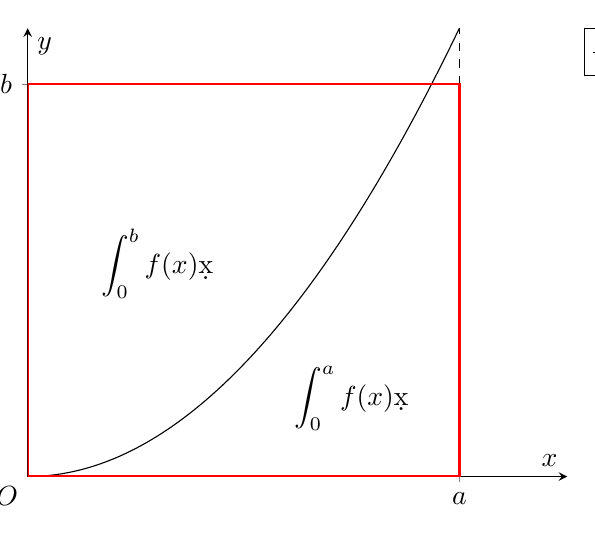
\begin{tikzpicture}[trim axis left, trim axis right]
            \begin{axis}[
                domain = 0:2.5,
                xmax = 2.5,
                restrict y to domain =0:4,
                samples = 101,
                axis y line=middle,
                axis x line=middle,
                xtick = {2},
                xticklabels = {$a$},
                ytick = {3.5},
                yticklabels = {$b$},
                xlabel = {$x$},
                ylabel = {$y$},
                legend cell align={left},
                legend pos=outer north east,
                after end axis/.code={
                    \path (axis cs:0,0) 
                    node [anchor=north east] {$O$};
                    }
                ]
                \addplot[black] {x^2};
                \addlegendentry{$y = f(x)$};
                \node at (0.6, 1.9) {$\displaystyle\int_0^b \inv f(x) \d x$};
                \node at (1.5, 0.7) {$\displaystyle\int_0^a f(x) \d x$};
                \draw[dashed] (2, 3.5) -- (2, 4);
                \draw[thick, red] (0, 0) -- (2, 0) -- (2, 3.5) -- (0, 3.5) -- (0,0);
            \end{axis}
        \end{tikzpicture}
        \end{figure}
        The sum of the areas represented by the two integrals is bigger than the area of the rectangle, $ab$.
    \end{ppart}
    \begin{ppart}
        Take $f(x) = x^{p-1}$, which is strictly increasing with $f(0) = 0$. Note that $\inv f(x) = x^{1/(p-1)}$. By (a), for all $a, b > 0$, \[ab \leq \int_0^a x^{p-1} \d x + \int_0^b x^{\frac1{p-1}} \d x = \frac{a^p}{p} + \frac{p-1}{p} b^{\frac{p}{p-1}} = \frac{a^p}{p} + \frac{a^q}{q},\] where $q = p/(p-1)$. Note that we indeed have $1/p + 1/q = 1$: \[q = \frac{p}{p-1} \implies \frac1q + \frac{p-1}p = 1 - \frac1p \implies \frac1p + \frac1q = 1.\]

        Under the transformations $a \mapsto \abs{a}/c$, $b \mapsto \abs{b}/{d}$, we see that \[\frac{\abs{ab}}{cd} \leq \frac{\abs{a}^p}{c^p p} + \frac{\abs{b}^q}{d^q q}\] for all $a, b \in \RR$ and $c, d > 0$.
    \end{ppart}
    \begin{ppart}
        \begin{psubpart}
            The triangle inequality states that $\abs{c_i} + \abs{d_i} \geq \abs{c_i + d_i}$. So \[\sum_{i = 1}^m \bs{\bp{\abs{c_i} + \abs{d_i}} \abs{c_i + d_i}^{p-1}} \geq = \sum_{i = 1}^m \abs{c_i + d_i} \abs{c_i + d_i}^{p-1} = \sum_{i = 1}^m \abs{c_i + d_i}^p.\]
        \end{psubpart}
        \begin{psubpart}
            Since $q = p/(p-1)$, we trivially have $q(p-1) = p$.
        \end{psubpart}
        \begin{psubpart}
            From (a), 
            \begin{align*}
                \sum_{i = 1}^m \abs{c_i + d_i}^p &\leq \sum_{i = 1}^m \bs{\bp{\abs{c_i} + \abs{d_i}} \abs{c_i + d_i}^{p-1}}\\
                &= \sum_{i = 1}^m \abs{c_i} \abs{c_i + d_i}^{p-1} + \sum_{i = 1}^m \abs{d_i} \abs{c_i + d_i}^{p-1}.
            \end{align*}
            Applying H\"{o}lder's inequality on both sums, we see that
            \begin{align*}
                &\sum_{i = 1}^m \abs{c_i + d_i}^p\\
                &\hspace{1em}\leq \bp{\sum_{i = 1}^m \abs{c_i}^p}^{1/p} \bp{\sum_{i = 1}^m \abs{c_i + d_i}^{(p-1)q}}^{1/q} + \bp{\sum_{i = 1}^m \abs{d_i}^p}^{1/p} \bp{\sum_{i = 1}^m \abs{c_i + d_i}^{(p-1)q}}^{1/q}\\
                &\hspace{1em}= \bs{\bp{\sum_{i = 1}^m \abs{c_i}^p}^{1/p} + \bp{\sum_{i = 1}^m \abs{d_i}^p}^{1/p}}\bp{\sum_{i = 1}^m \abs{c_i + d_i}^{p}}^{1/q}
            \end{align*}
            Dividing both sides by $\bp{\sum_{i = 1}^m \abs{c_i + d_i}^{p}}^{1/q}$, we have our desired inequality: \[\bp{\sum_{i = 1}^m \abs{c_i + d_i}^p}^{1/p} = \bp{\sum_{i = 1}^m \abs{c_i + d_i}^p}^{1 - 1/q} \leq \bp{\sum_{i = 1}^m \abs{c_i}^p}^{1/p} + \bp{\sum_{i = 1}^m \abs{d_i}^p}^{1/p}.\]
        \end{psubpart}
        \begin{psubpart}
            Take $c \mapsto c w^{1/p}$, $d \mapsto d w^{1/p}$ and invoke (c)(ii).
        \end{psubpart}
    \end{ppart}
\end{solution}